\section{Numerical Results and Discussion}
\label{sec:numerical}
\subsection{Simulation Setup}
The synthetic HAP altitude is $20$ km and its horizontal position is
$(11419.6551,450)$ m. The UAV flies at $1$ km over 100 cell centers,
with coordinates $50,150,\ldots,950$ m along each axis (the $x$ index
changes first). The reference mission has $30$ slots of $20$ s and
$v_{\max}=15$ m/s, permitting transitions up to $300$ m.
These are simulation assumptions rather than measured deployment data.

The common P1 catalog contains 233 authenticated sources: 197
Maxwell--Boltzmann (MB) and 36 uniform ensembles. P1 selects
$(\nu,V_A)=(0.125,8)$ at all 100 positions, where $V_A=8$ is the upper
MB-catalog boundary. Thus, differences among positioning methods do
not arise from changing the selected shaping parameters. The saved
clear-sky rates range from $1.16296\times10^{-4}$ to
$1.57800\times10^{-4}$ bit/use. Table~\ref{tab:setup} lists the
retained optical and noise parameters. No numerical model or source
calculation is rerun for this revision.

\begin{table}[t]
\caption{Retained Synthetic Simulation Parameters}
\label{tab:setup}
\centering\footnotesize
\begin{tabular}{@{}p{0.54\columnwidth}p{0.40\columnwidth}@{}}
\toprule
Parameter & Value\\\midrule
Wavelength; full beam divergence & $1550$ nm; $233\,\mu$rad\\
Receiver diameter; zenith transmission & $0.08$ m; $0.92$\\
Angular jitter; horizontal jitter & $15.61\,\mu$rad; $1$ m\\
Boresight displacement & $0$ m\\
AoA standard deviation; FOV half angle & $1.5$ mrad; $6.25$ mrad\\
Hufnagel--Valley wind speed & $21$ m/s\\
Ground-level $C_n^2(0)$ & $10^{-14}\,\mathrm{m}^{-2/3}$\\
$\beta_{\rm rec}$; $\xi_{\rm ch}$ & $0.95$; $0.0186$ SNU\\
Detector efficiency; electronic noise & $1$; $0$\\
Default $p$; $\ell$; latent $\rho$ & $0.4$; $250$ m; $0.9$\\
Independent mission IDs & $0,\ldots,99$\\
Reference distance $D_{\rm ref}$ & $1000$ m\\\bottomrule
\end{tabular}
\end{table}

The saved complete-blockage model thresholds a stationary Gaussian
field: its spatial covariance is $\Sigma_{ij}=\exp(-d_{i,j}/\ell)$ and
$\mathbf z_n=\rho\mathbf z_{n-1}+\sqrt{1-\rho^2}\boldsymbol\epsilon_n$,
where $\boldsymbol\epsilon_n\sim\mathcal N(0,\Sigma)$ and
$\mathbf z_1\sim\mathcal N(0,\Sigma)$. Blockage is
$c_{j,n}=\mathbb I\{z_{j,n}<\Phi^{-1}(p)\}$.
The seed is 20261015 with mission IDs 0--99. Configurations share
innovations for paired comparisons. Latent $\rho$ and $\ell$ are
distinct from binary-cloud correlations. Unless varied,
$(p,\ell,\rho)=(0.4,250\,\mathrm m,0.9)$.

For a path $\mathbf j=(j_1,\ldots,j_{N_t})$, we report
\begin{align}
 \overline K(\mathbf j)&=\frac{1}{N_t}\sum_{n=1}^{N_t}S_{j_n,n},
 \label{eq:mean_skr}\\
 D(\mathbf j)&=\sum_{n=2}^{N_t}d_{j_{n-1},j_n},\label{eq:distance}\\
 U(\mathbf j)&=\overline K(\mathbf j)-\lambda D(\mathbf j)/D_{\rm ref}.
 \label{eq:utility}
\end{align}
Availability is $N_t^{-1}\sum_n\mathbb I\{S_{j_n,n}>0\}$;
unavailability is its complement, expressed in percent. This nonzero-rate
definition has no positive engineering threshold. The reference penalty
is the fixed absolute value
$\lambda_{\rm ref}=9.468026677248516\times10^{-6}$ bit/use.
The ten saved penalties have multipliers
$\{0,10^{-4},3\times10^{-4},10^{-3},3\times10^{-3},10^{-2},
3\times10^{-2},0.1,0.3,1\}$ of
$\lambda_{\rm hi}=0.003156008892416172$ bit/use; thus
$\lambda_{\rm ref}=0.003\lambda_{\rm hi}$.

Means use 100 independent missions per configuration. Pointwise 95\%
percentile-bootstrap intervals resample whole missions with 20000
replicates; paired method contrasts use the same mission IDs. Saved
intervals are retained, and missing tradeoff intervals use saved metrics
and existing resampling counts. These intervals quantify mission
variability, not quantum-security uncertainty. The multi-curve
presentation is informed by~\cite{gong2020}; its satellite model and
numerical results are not transferred to this experiment.

\subsection{Impact of Candidate UAV Positions}
Figure~\ref{fig:positions} compares deterministic nested subsets
$J=10,20,40,60,80,100$ at $\lambda_{\rm ref}$. The mean DP objective
increases from $1.39004\times10^{-4}$ to $1.54863\times10^{-4}$ bit/use,
an $11.41\%$ increase relative to $J=10$. P2 increases from
$1.36348\times10^{-4}$ to $1.50243\times10^{-4}$, and Greedy from
$1.07800\times10^{-4}$ to $1.48311\times10^{-4}$ bit/use.
Adding positions preserves existing feasible paths, so optimal P2 and
DP objectives cannot decrease; Greedy has no such general guarantee.

At $J=20$, DP reaches $96.71\%$ of its $J=100$ objective. However,
the $J=10$ transition graph has eight connected components and seven
isolated positions, whereas the sampled subsets are connected from
$J=20$ onward. The initial improvement combines expanded spatial
choices and connectivity changes; it does not identify an economically
optimal grid size or isolate candidate density alone.

\begin{figure*}[!t]
\centering
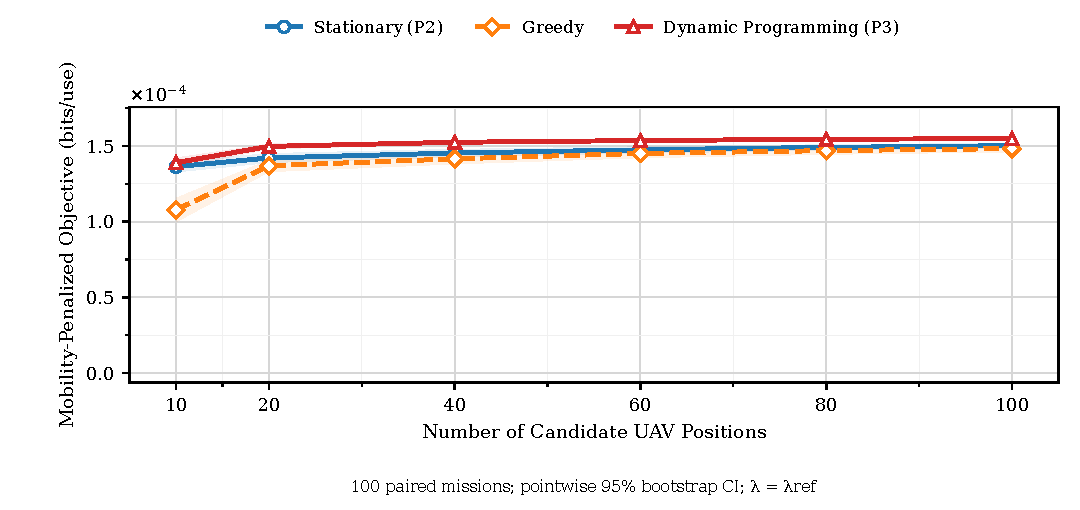
\includegraphics[width=\textwidth]{figures/fig1_candidate_positions.pdf}
\caption{Mean mobility-penalized objective versus the number of candidate
UAV positions at $\lambda_{\rm ref}$. Stationary (P2), Greedy, and DP
use deterministic nested subsets of the original coordinates and common
cloud missions. Shaded bands show pointwise 95\% whole-mission bootstrap
intervals. The objective includes a distance penalty and is distinct
from average usable SKR.}
\label{fig:positions}
\end{figure*}

\subsection{Impact of Cloud Blockage Probability}
Figure~\ref{fig:probability}(a) shows decreasing mean usable SKR as
$p$ increases from $0.1$ to $0.8$ for all three methods. DP decreases
from $1.57663\times10^{-4}$ to $1.43475\times10^{-4}$ bit/use.
The probability masks are nested under common innovations: increasing
$p$ removes usable rewards. Therefore, the optimal P2 and DP
\emph{objectives} cannot increase; a general availability or Greedy
ordering does not follow.

The DP-minus-P2 mean objective difference grows from
$1.11215\times10^{-7}$ to $2.72806\times10^{-5}$ bit/use. Dividing
each difference by its corresponding P2 mean gives gains of $0.071\%$
and $25.042\%$. At $p=0.8$, the paired 95\% interval for the absolute
difference is $[2.46760,2.99896]\times10^{-5}$ bit/use. The larger
relative gain is consequently accompanied by a larger absolute gain.
No interior maximum occurs on the evaluated probability grid, and no
claim is made beyond $p=0.8$.

In Fig.~\ref{fig:probability}(b), unavailability at $p=0.8$ is $24.60\%$
for P2, $16.53\%$ for Greedy, and $4.07\%$ for DP. These observed
availability benefits do not mean that P3 maximizes availability.
Greedy's mean objective is below P2 at $p=0.1$--$0.4$; its paired
differences at $p=0.5$ and $0.7$ have intervals containing zero.
At $p=0.8$, its objective exceeds P2 by $8.54160\times10^{-6}$ bit/use,
less than DP's improvement.

\begin{figure*}[!t]
\centering
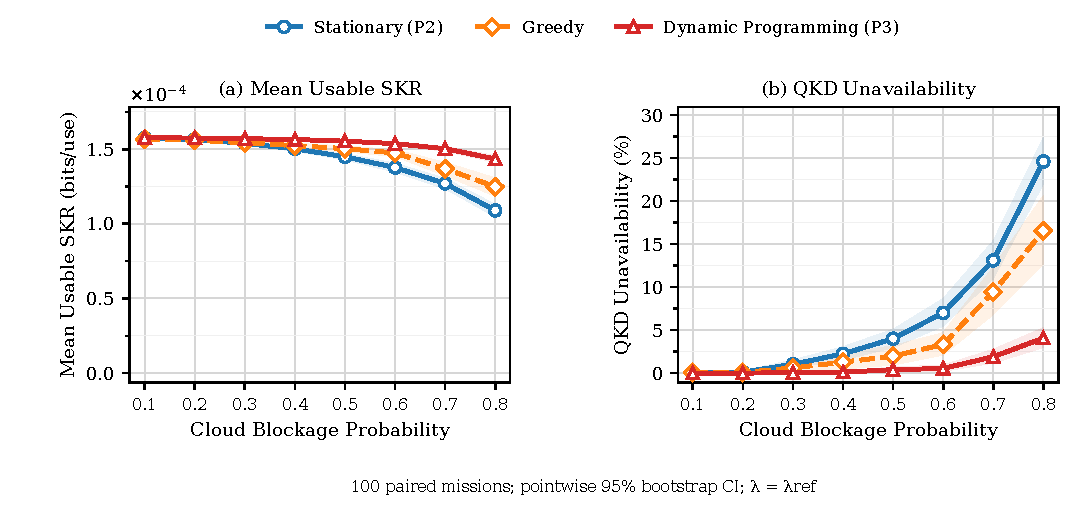
\includegraphics[width=\textwidth]{figures/fig2_cloud_blockage.pdf}
\caption{Cloud-blockage sensitivity at $\lambda_{\rm ref}$:
(a) mean usable SKR and (b) zero-SKR unavailability for P2, Greedy,
and DP. All eight probabilities $p=0.1,0.2,\ldots,0.8$ use 100 paired
missions with common innovations. Bands are pointwise 95\%
whole-mission bootstrap intervals. Unavailability counts zero usable
SKR, without an engineering threshold; neither panel is the optimized
penalized objective.}
\label{fig:probability}
\end{figure*}

\subsection{Impact of Temporal Cloud Correlation}
Figure~\ref{fig:temporal} varies latent
$\rho\in\{0,0.3,0.6,0.9,0.98\}$ at $p=0.4$, $\ell=250$ m, and
$\lambda_{\rm ref}$. From $\rho=0$ to $0.98$, DP's mean objective
increases from $1.44559\times10^{-4}$ to $1.56806\times10^{-4}$ bit/use,
while its mean distance decreases from $1038.25$ to $31.84$ m.
Its relative objective gain over P2 falls from $23.712\%$ to $0.155\%$.

Saved-mask diagnostics support a persistence explanation. The
cloud-free fraction at the selected P2 location rises from $77.03\%$
to $99.97\%$, and the mean number of locations clear throughout the
30-slot mission rises from zero to $29.56$. The global fraction of
adjacent cell-slot states that change falls from $48.21\%$ to $6.35\%$.
DP's mean number of moves decreases from $7.36$ to $0.19$; missions
containing DP movement decrease from 100 to 10 out of 100.

Persistent favorable locations therefore make offline stationary
selection more competitive in this experiment. This is a supported
mechanism, not an isolated causal result or universal monotonic law.
P2 and DP choose initial positions using future clouds, whereas Greedy
does not. At $\rho=0.98$, the latent correlation time
$-20/\log\rho\simeq990$ s exceeds the 600-s mission. Empirical
blockage varies across the finite samples despite fixed nominal $p$.

\begin{figure*}[!t]
\centering
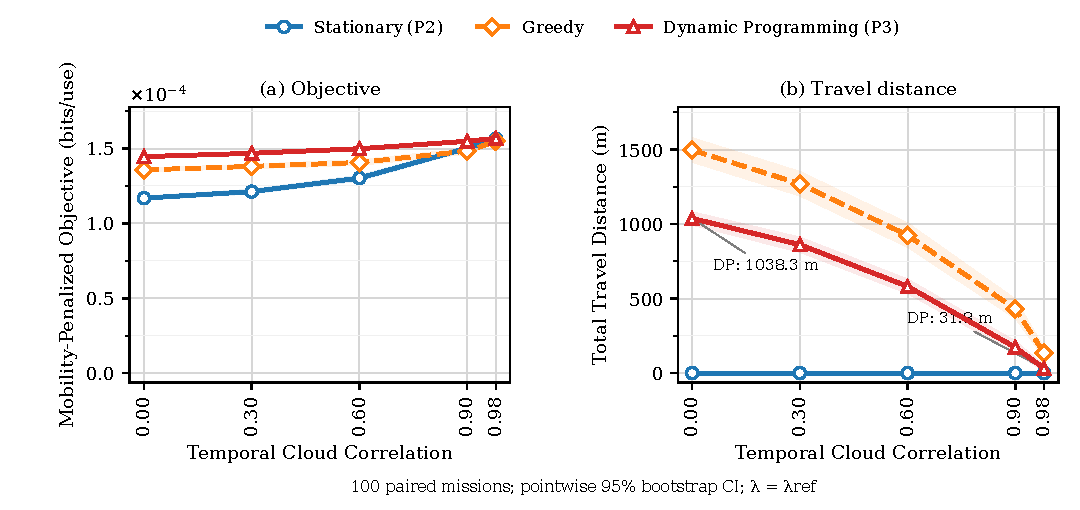
\includegraphics[width=\textwidth]{figures/fig3_temporal_correlation.pdf}
\caption{Latent temporal-correlation sensitivity: (a) mean penalized
objective and (b) mean total travel distance at $p=0.4$, $\ell=250$ m,
and $\lambda_{\rm ref}$. P2, Greedy, and DP share 100 mission IDs and
common innovations. P2 and DP know the full horizon; Greedy uses the
current slot. The latent coefficient differs from binary blockage
correlation. Bands are pointwise 95\% whole-mission bootstrap intervals.}
\label{fig:temporal}
\end{figure*}

\subsection{SKR--Mobility Tradeoff}
Figure~\ref{fig:tradeoff} connects saved policies in the original order
of ten increasing penalties. At $\lambda=0$, DP achieves mean usable
SKR $1.57305\times10^{-4}$ bit/use and distance $1482.69$ m. At
$\lambda_{\rm ref}$, distance falls to $172.43$ m and mean SKR to
$1.56495\times10^{-4}$ bit/use. Relative to the respective zero-penalty
means on the same 100 default missions, these changes are an
$88.37\%$ distance reduction and a $0.515\%$ SKR reduction.

At $\lambda_{\rm ref}$, Greedy travels $430.61$ m, while DP has both
higher mean SKR and higher objective. DP's SKR gains relative to P2
and Greedy are $4.162\%$ and $2.695\%$; its objective gains are
$3.075\%$ and $4.418\%$, respectively. The paired DP-minus-P2
objective interval is $[3.56503,5.73139]\times10^{-6}$ bit/use.
The distinction matters because movement is penalized only in $U$.

At sampled penalties $0.1\lambda_{\rm hi}$ and above, all saved DP
paths are stationary and coincide with P2 in objective. This does not
identify a continuous stopping threshold. Greedy can stop at a worse
location because it chooses its initial position from the first slot.
Optimal DP distance is nonincreasing with $\lambda$ for the same
feasible set and rewards; the plotted points are evaluated numerical
operating choices, not global physical Pareto frontiers.

\begin{figure*}[!t]
\centering
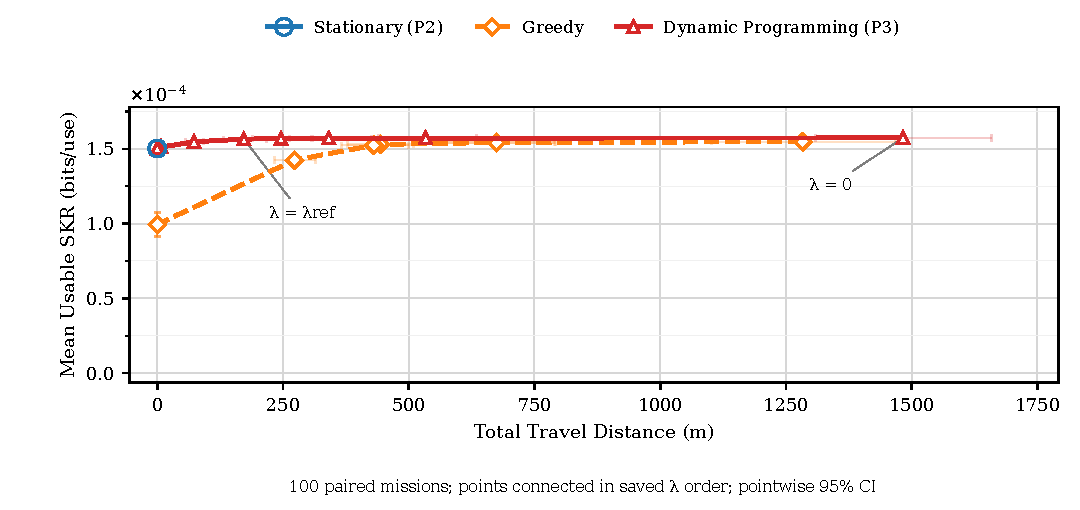
\includegraphics[width=\textwidth]{figures/fig4_skr_mobility_tradeoff.pdf}
\caption{Evaluated usable-SKR--distance tradeoff for Greedy and DP,
with P2 as the stationary reference, under default clouds. Curves
connect the ten saved penalties in their original increasing order;
DP annotations identify zero and representative penalties. Error bars
are pointwise 95\% intervals for each mean, not joint confidence
regions. Coincident high-penalty DP points and the P2 reference are
retained. These conditional model outputs are not claimed to be
global physical Pareto frontiers.}
\label{fig:tradeoff}
\end{figure*}

\subsection{Discussion and Limitations}
Across the investigated parameter ranges, the largest mean-SKR span
occurs for candidate count in DP, speed in Greedy, and blockage
probability in P2. These are descriptive ranges over unequal domains,
not normalized sensitivity indices. Among cloud sweeps, the largest
relative DP-versus-P2 objective gain occurs at $p=0.8$, while the
largest absolute difference occurs at $\rho=0$. The supplementary
spatial sweep also distinguishes absolute performance from mobility
gain: increasing $\ell$ from $50$ to $1000$ m reduces absolute
performance but increases the DP-minus-P2 objective difference from
$2.25288\times10^{-6}$ to $8.10831\times10^{-6}$ bit/use. Full-grid
blockage grows from zero to $2.70\%$ of slots. A larger relative gain
therefore does not imply increasing spatial diversity.

P1 provides the common catalog-selected map, P2 captures offline
fixed-position selection, and DP-minus-P2 measures the extra value
of permitting movement in that setting. Since all positions select
the same source, cloud-avoidance gains cannot be assigned to adaptive
shaping. These three methods do not isolate matched-energy shaping
gain or stationary-selection gain relative to a fixed deployment.
DP-minus-Greedy includes differences in future-state and initial-position
information. Objective dominance does not imply higher SKR in every
positive-penalty mission.

The study is restricted to a finite source catalog and UAV grid,
synthetic weather and geometry, and complete cloud blockage. Tracking
interruptions, reacquisition, deployment, return travel, and calibrated
propulsion energy are omitted. The mixed 2D-MI/homodyne model in
Section~\ref{sec:security}, the effective-likelihood approximation,
and correlation-domain treatment prevent a validated physical SKR
interpretation. Trusted receiver noise would require a separate
consistent model~\cite{usenko2016}. Asymptotic rate arithmetic and
mission confidence intervals establish neither operational nor
finite-key, composable, or unconditional security.
